\documentclass[10pt, xcolor=dvipsnames]{beamer}

% There are many different themes available for Beamer. A comprehensive
% list with examples is given here:
% http://deic.uab.es/~iblanes/beamer_gallery/index_by_theme.html
% You can uncomment the themes below if you would like to use a different
% one:
%\usetheme{AnnArbor}
%\usetheme{Antibes}
%\usetheme{Bergen}
%\usetheme{Berkeley}
%\usetheme{Berlin}
%\usetheme{Boadilla}
%\usetheme{boxes}
%\usetheme{CambridgeUS}
%\usetheme{Copenhagen}
%\usetheme{Darmstadt}
%\usetheme{default}
%\usetheme{Frankfurt}
%\usetheme{Goettingen}
%\usetheme{Hannover}
%\usetheme{Ilmenau}
%\usetheme{JuanLesPins}
%\usetheme{Luebeck}
%\usetheme{Frankfurt}
\usetheme{Madrid}
%\usetheme{Malmoe}
%\usetheme{Marburg}
%\usetheme{Montpellier}
%\usetheme{PaloAlto}
%\usetheme{Pittsburgh}
%\usetheme{Rochester}
%\usetheme{Singapore}
%\usetheme{Szeged}
%\usetheme{Warsaw}

\usepackage[utf8]{inputenc}
\usepackage[english]{babel}
\usepackage{ragged2e}
\usepackage{bbding}
%\usepackage{enumitem}
\usepackage{mathtools}
\usepackage{indentfirst}
\usepackage{graphicx}
\usepackage{float}
\usepackage{hyperref}
\usepackage{mathtools}
\usepackage{preview}
\usepackage{xcolor}
\usepackage{color}
\usepackage{listings}
\usepackage{float}
\usepackage[caption = false]{subfig}
\usepackage{pdfpages}
\usepackage{multirow}
\usepackage{array}
\usepackage{makecell}
\usepackage{bm}
\usepackage{caption}
\usepackage{cancel}
\usepackage{anyfontsize}
\usepackage{etoolbox}
\usepackage{amsmath}
\usepackage{amssymb}
\usepackage{mathtools}
\usepackage{natbib}
\usepackage[flushleft]{threeparttable}
\usepackage{booktabs}
\usepackage{caption}
\usepackage{adjustbox}
\usepackage{appendixnumberbeamer}
\usepackage{pifont}
\usepackage{amsmath}
\usepackage{amssymb}
\usepackage[percent]{overpic}



\setbeamercolor{titlelike}{parent=structure}
\definecolor{UBCblue}{rgb}{0.04706, 0.13725, 0.32}
\colorlet{UBCblue2}{UBCblue!70!white}
\usecolortheme[named=UBCblue]{structure}

\makeatletter
\setbeamertemplate{footline}
{
  \leavevmode%
  \hbox{%
  \begin{beamercolorbox}[wd=.4\paperwidth,ht=2.25ex,dp=1ex,center]{author in head/foot}%
    \usebeamerfont{author in head/foot} \insertshortauthor %\hspace*{1em}(\insertshortinstitute)
  \end{beamercolorbox}%
  \begin{beamercolorbox}[wd=.5\paperwidth,ht=2.25ex,dp=1ex,center]{title in head/foot}%
    \usebeamerfont{title in head/foot} \insertshorttitle
  \end{beamercolorbox}%
  \begin{beamercolorbox}[wd=.1\paperwidth,ht=2.25ex,dp=1ex,center]{date in head/foot}%
    \usebeamerfont{date in head/foot}
    \insertframenumber{} / \inserttotalframenumber\hspace*{2ex} 
  \end{beamercolorbox}}%
  \vskip0pt%
}
\makeatother

\renewcommand{\arraystretch}{1.2}
\renewcommand{\raggedright}{\leftskip=0pt \rightskip=0pt plus 0cm}
\newcolumntype{C}[1]{>{\centering\let\newline\\\arraybackslash\hspace{0pt}}m{#1}}

\hypersetup{
    colorlinks=true,
    linkcolor=UBCblue,
    citecolor=UBCblue,
    filecolor=magenta,      
    urlcolor=blue,
    allcolors=.
}
\setbeamercolor{button}{bg=UBCblue2,fg=white}
\newcommand\fnote[1]{\captionsetup{font=tiny}\caption*{#1}}
\newcommand\fnotev[1]{\captionsetup{font=scriptsize}\caption*{#1}}
\setbeamertemplate{caption}[numbered]


%\justifying
\urlstyle{same}
%\usefonttheme{serif}

%------------------------
%------------------------

\date{}

%------------------------
%------------------------
%----------------------------------------------------------------------------------------
%	TITLE PAGE
%----------------------------------------------------------------------------------------------------------------
%------------------------

\title[Landlord Responses to Changes in Tenant Protections]{Are Slumlords Necessary: \\Landlord Responses to Changes in Tenant Protections} % The short title appears at the bottom of every slide, the full title is only on the title page
\author[Joe Fish]{Joe Fish}


\begin{document}

\begin{frame}
\titlepage % Print the title page as the first slide
\end{frame}

\begin{frame}{Motivation}

\begin{itemize}
    \item Most US cities have awful tenant protections
    \item Tenants perceived as risky face large barriers to finding housing. Lots of rental listings will have "no eviction, no conviction" clauses, effectively locking them out of large parts of the rental market. This is true for private and public landlords.
    \item Landlords that rent to risky tenants are providing a service, these landlords are also much more likely to be predatory.
    \item When advocacy groups push for stronger tenant protections, landlords (public and private) argue that increased tenant protections would make them unable to be effective landlords. Thus, it's ex ante, unclear what the best way to regulate low income landlords is.
\end{itemize}
\end{frame}


\begin{frame}{Research questions}

Do landlords actually respond to changes in tenant protections, and if so, how?\\
\vspace{0.5cm}
\textbf{Big Picture:} \\
\vspace{0.5cm}
Are slumlords just predatory, or are they providing "housing of last resort" by renting to tenants who would otherwise be screened out by the rest of the market (or a little bit of both) \\
\vspace{0.5cm}
Are the tenants ending up in these properties just unlucky victims or are they getting access to housing they might otherwise not

\end{frame}

\begin{frame}{Desired Feedback}
\begin{itemize}
    \item Framing and research question
    \item IO Side: what are the possible responses of the low income landlords
    \item How to do the empirics
    \item How to model selection into high eviction homes
\end{itemize}
    
\end{frame}

\begin{frame}{Philly post-COVID}
Post COVID, Philadelphia has seen one of the largest reductions in evictions in the country. \\
\vspace{0.5cm}
To some extent, this can be attributed to their eviction diversion program, which made it harder to evict tenants. \\
\vspace{0.5cm}
Given that Philly is a poor city with a substantial Black population that experienced a large change in tenant protections, it's the ideal place to look for changes in landlord behavior. \\
\vspace{0.5cm}
Other benefits: Rental registry, evictions have contract rent (means I can see low income rent prices), good historical data.
    
\end{frame}

\begin{frame}{Evictions in Philly: Time Series}
    \begin{figure}
    \centering
    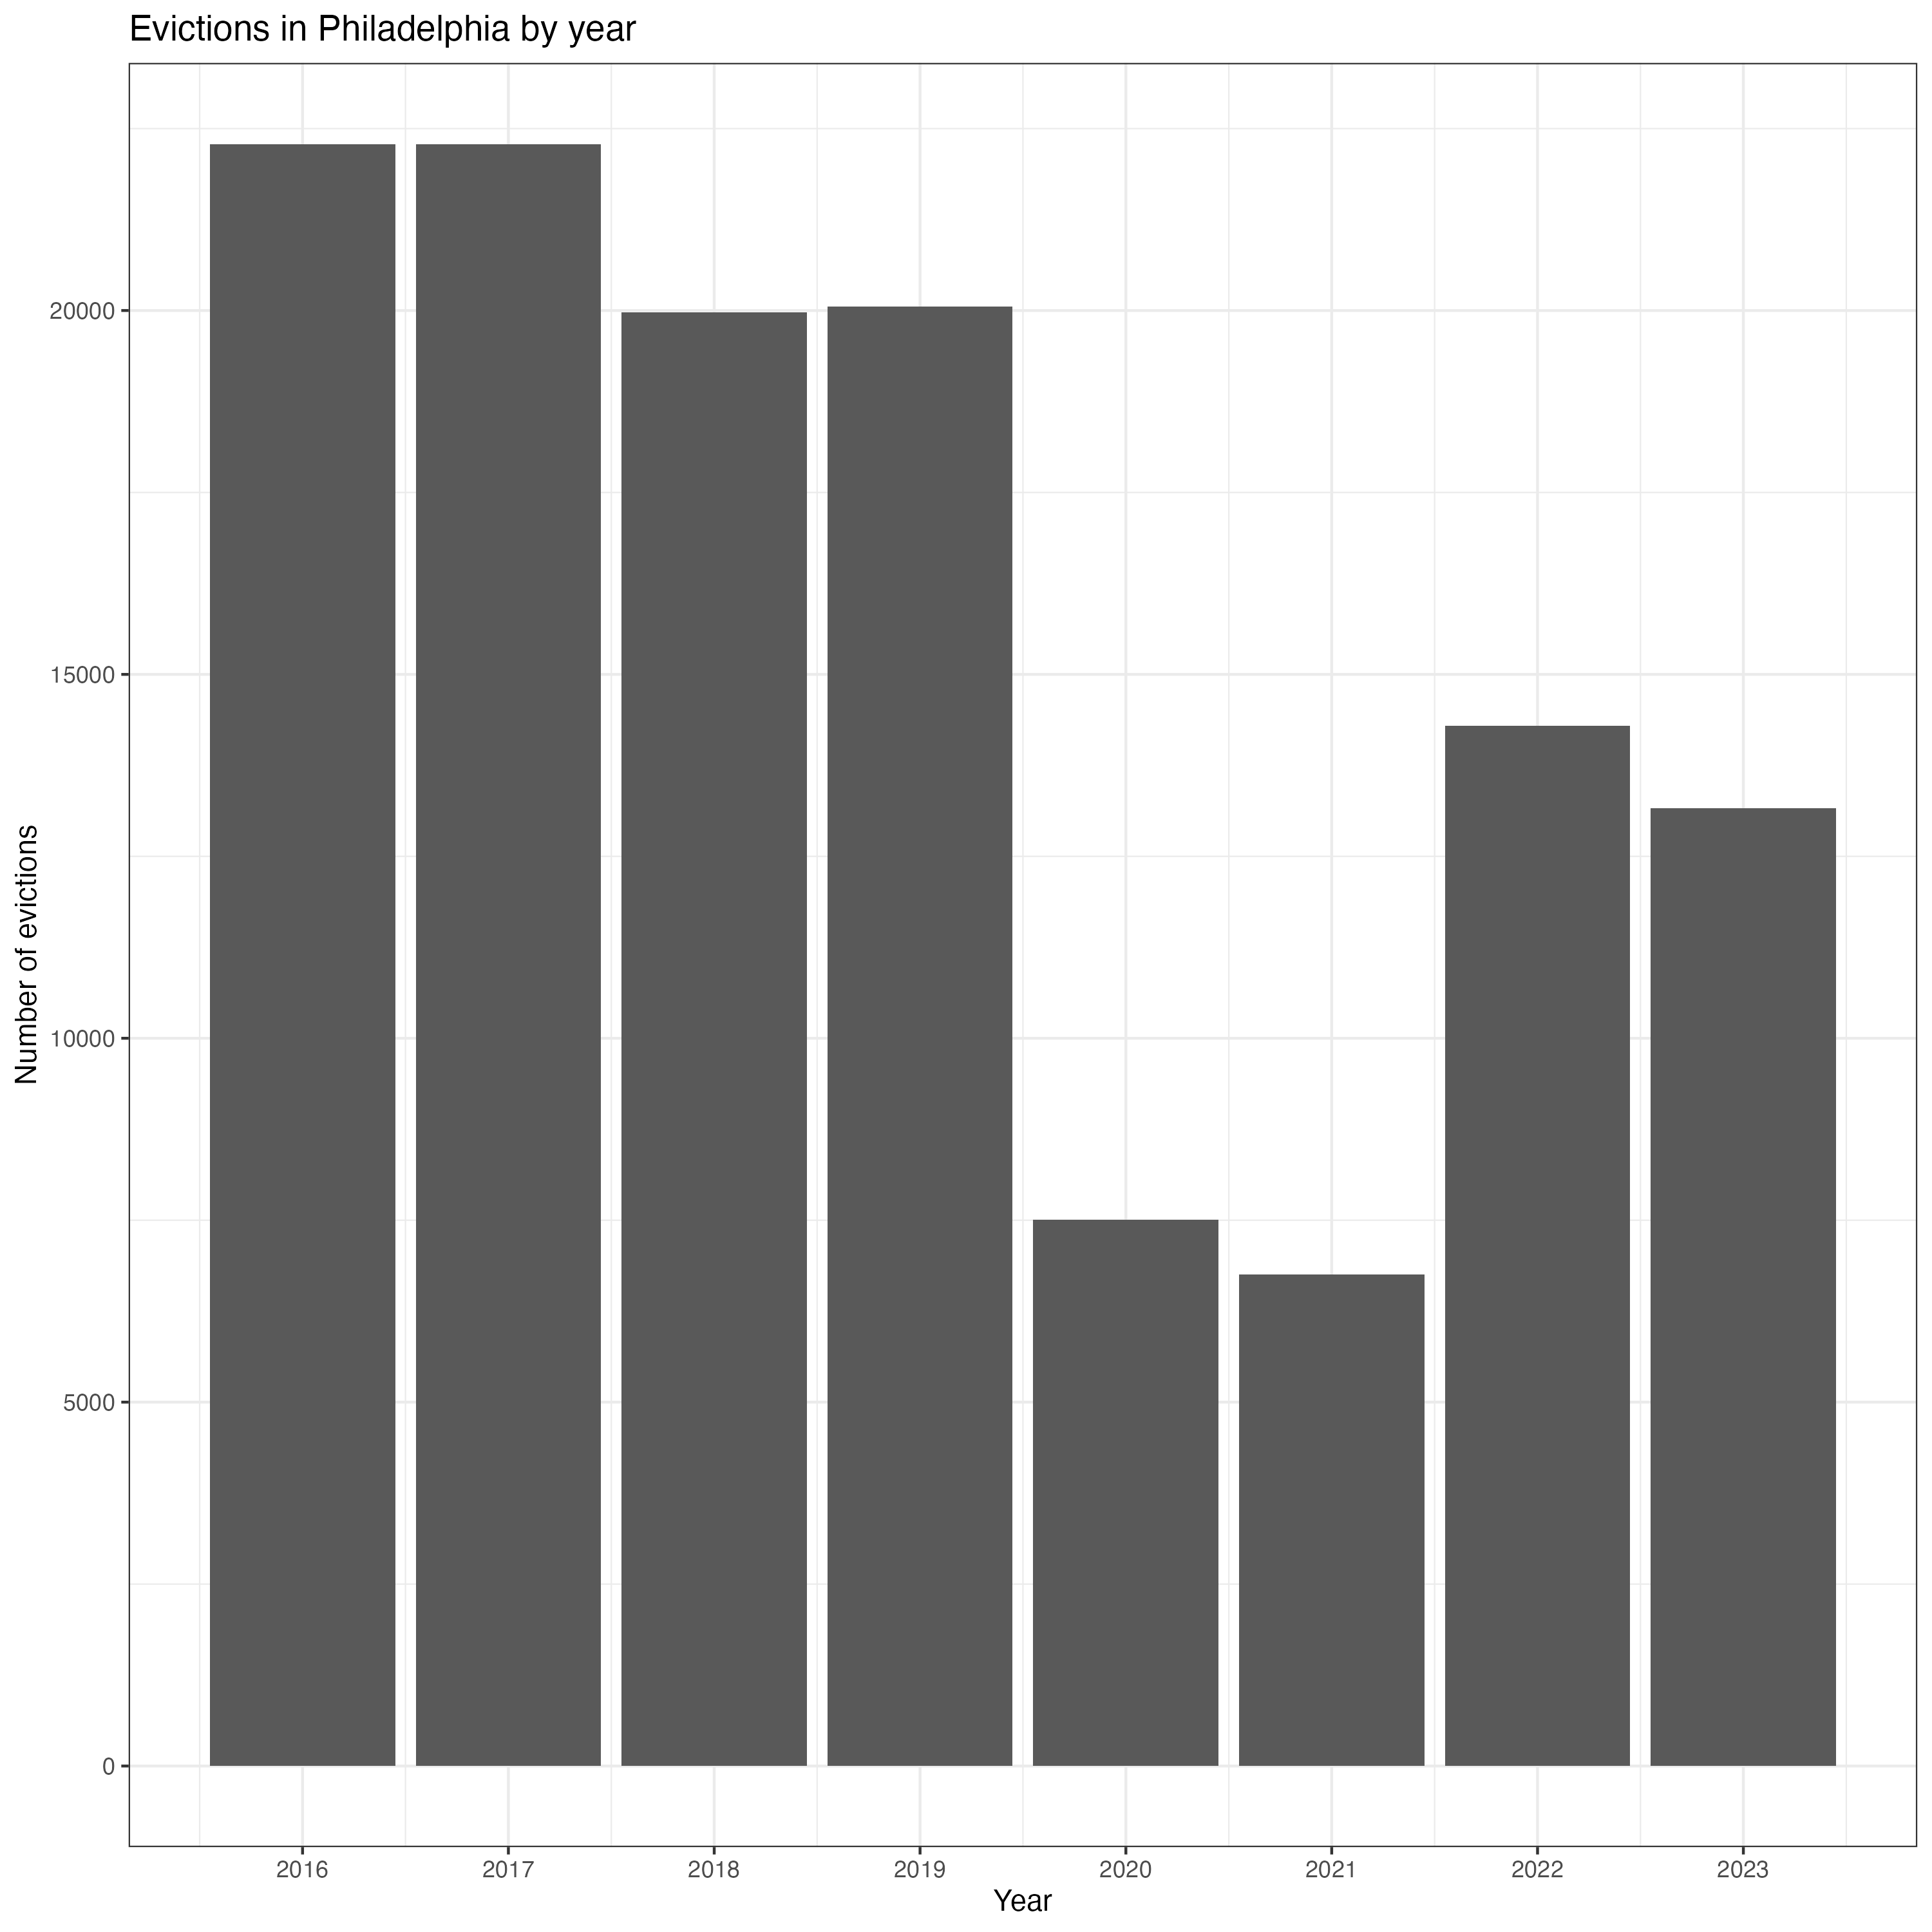
\includegraphics[width=0.5\linewidth]{figs/evict_by_year.png}
    \caption{Evictions in Philadelphia by Year}
    \label{fig:philly-ts}
\end{figure}
\end{frame}


\begin{frame}{Evictions in America}
\textbf{Evictions in America are heavily concentrated:}
\begin{itemize}
    \item They are concentrated within certain cities (poorer, Blacker ones)
    \item Within cities, they are concentrated within certain neighborhoods (poorer, Blacker ones)
    \item Within neighborhoods, they are concentrated within certain buildings and within specific landlords 
\end{itemize} 

    
\end{frame}

\begin{frame}{Evictions in America: National}
\begin{figure}
    \centering
    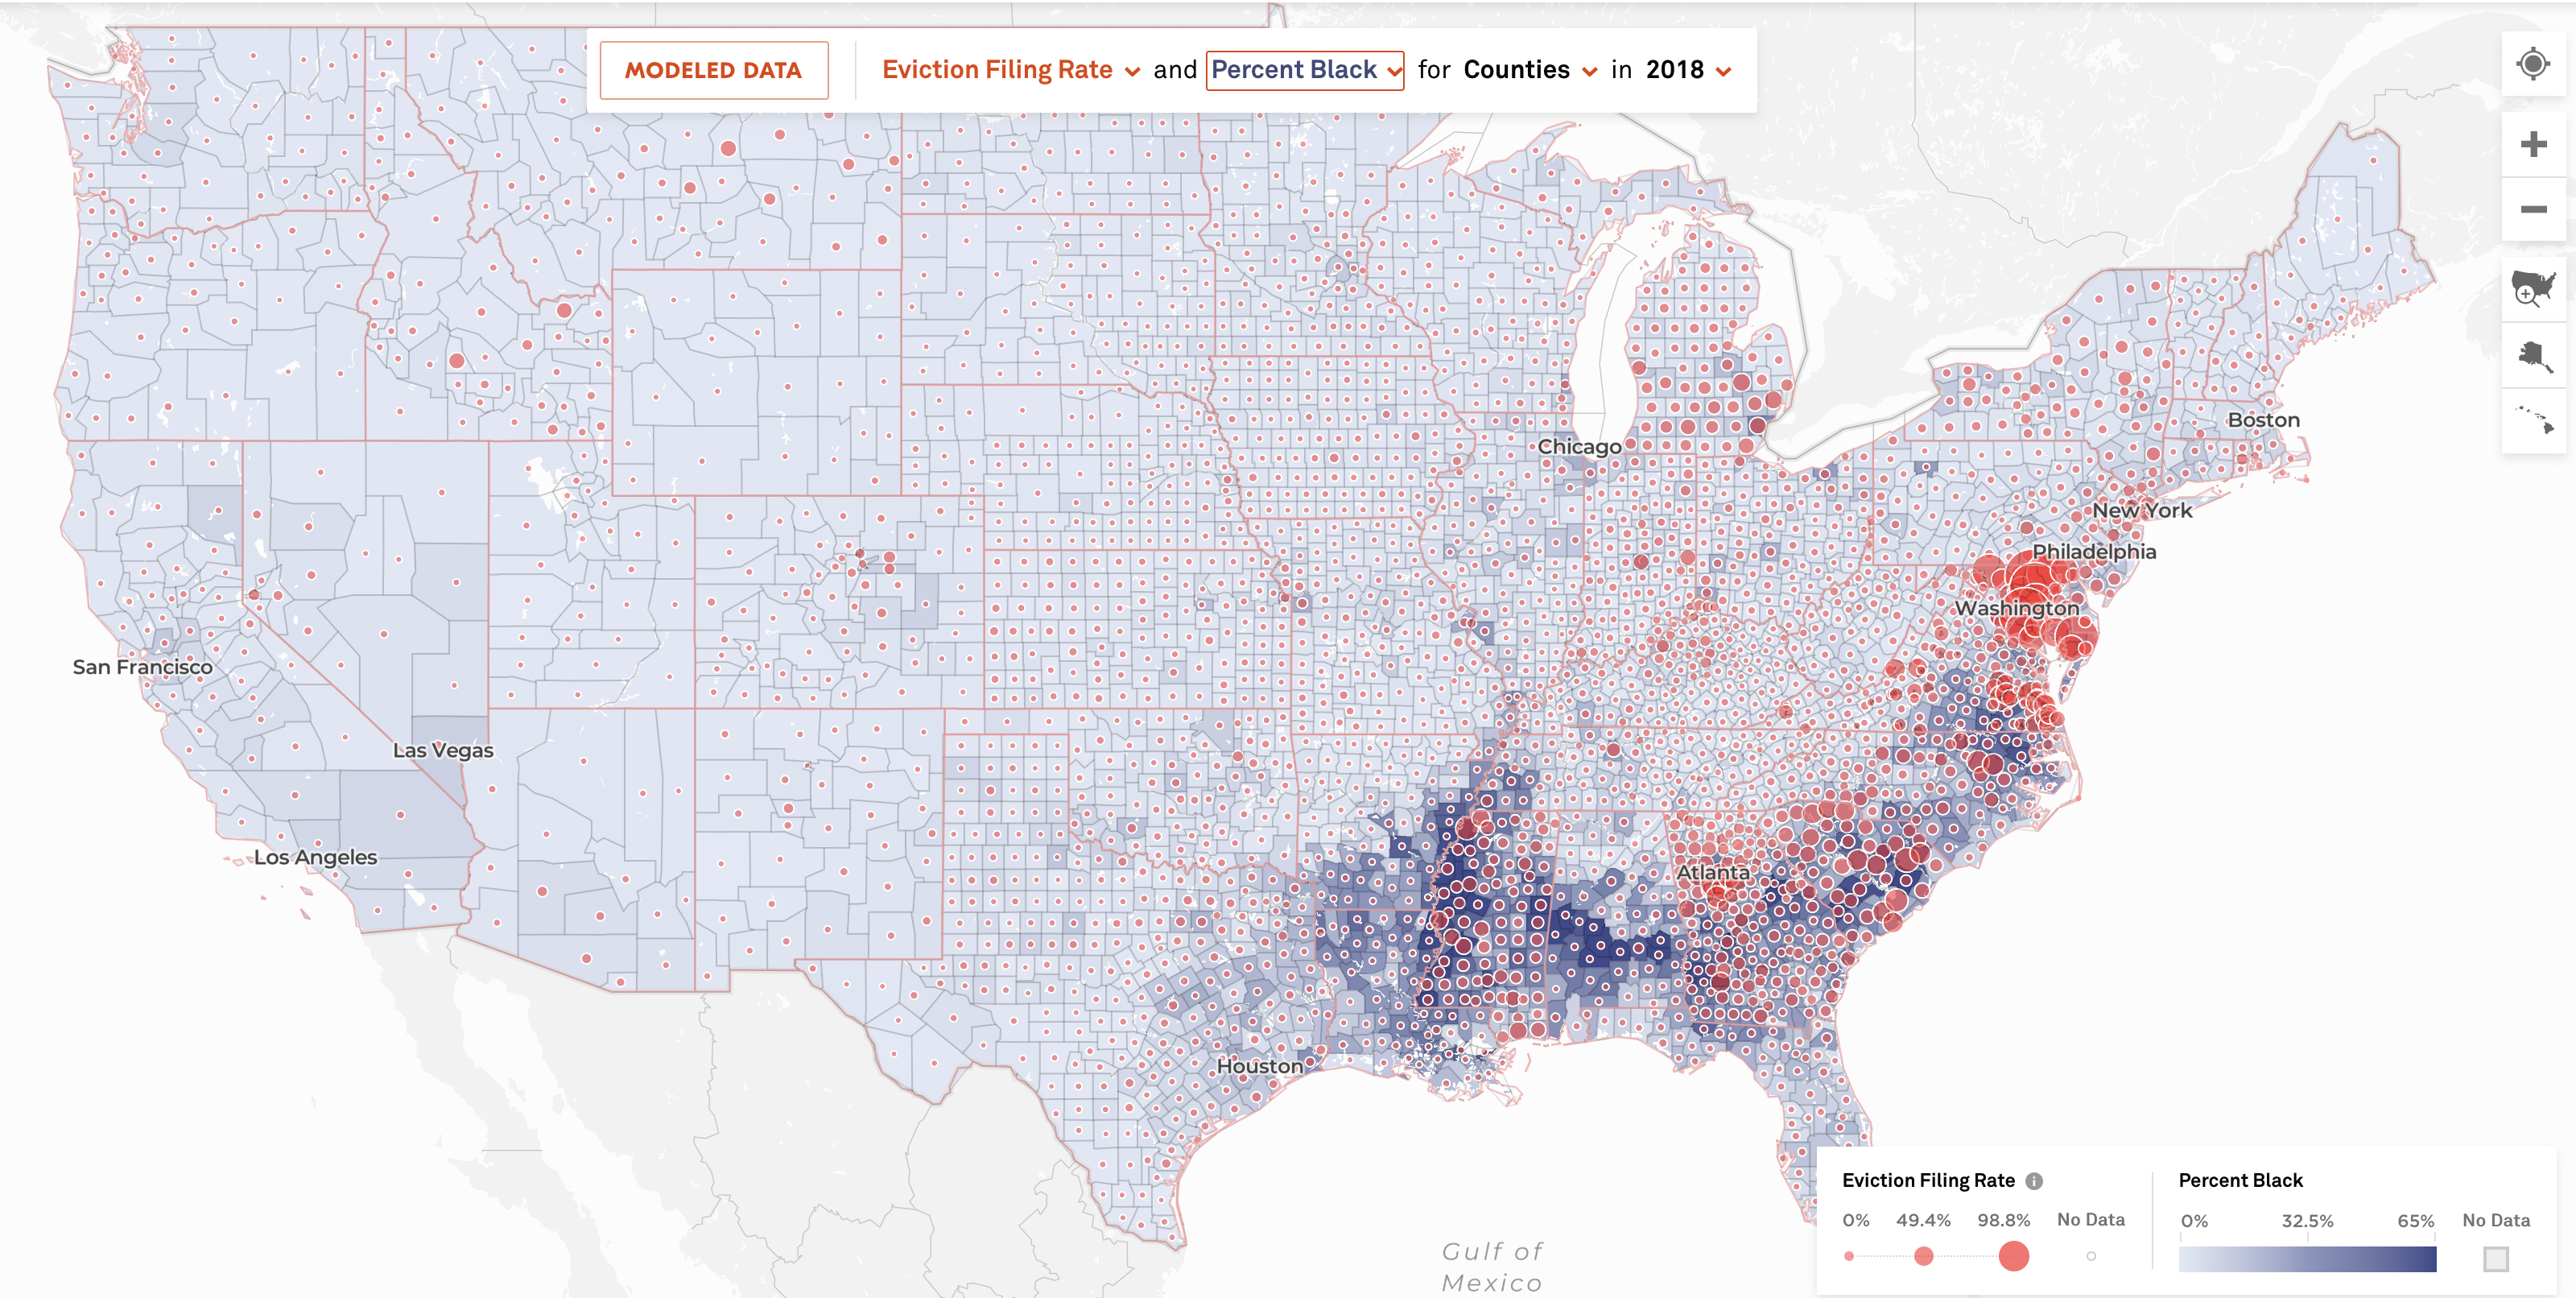
\includegraphics[width=0.65\linewidth]{figs/national-eviction-map.png}
    \caption{Evictions in America}
    \label{fig:natl-map}
\end{figure}
    
\end{frame}


\begin{frame}{Evictions in Philadelphia: Map}
\begin{figure}
    \centering
    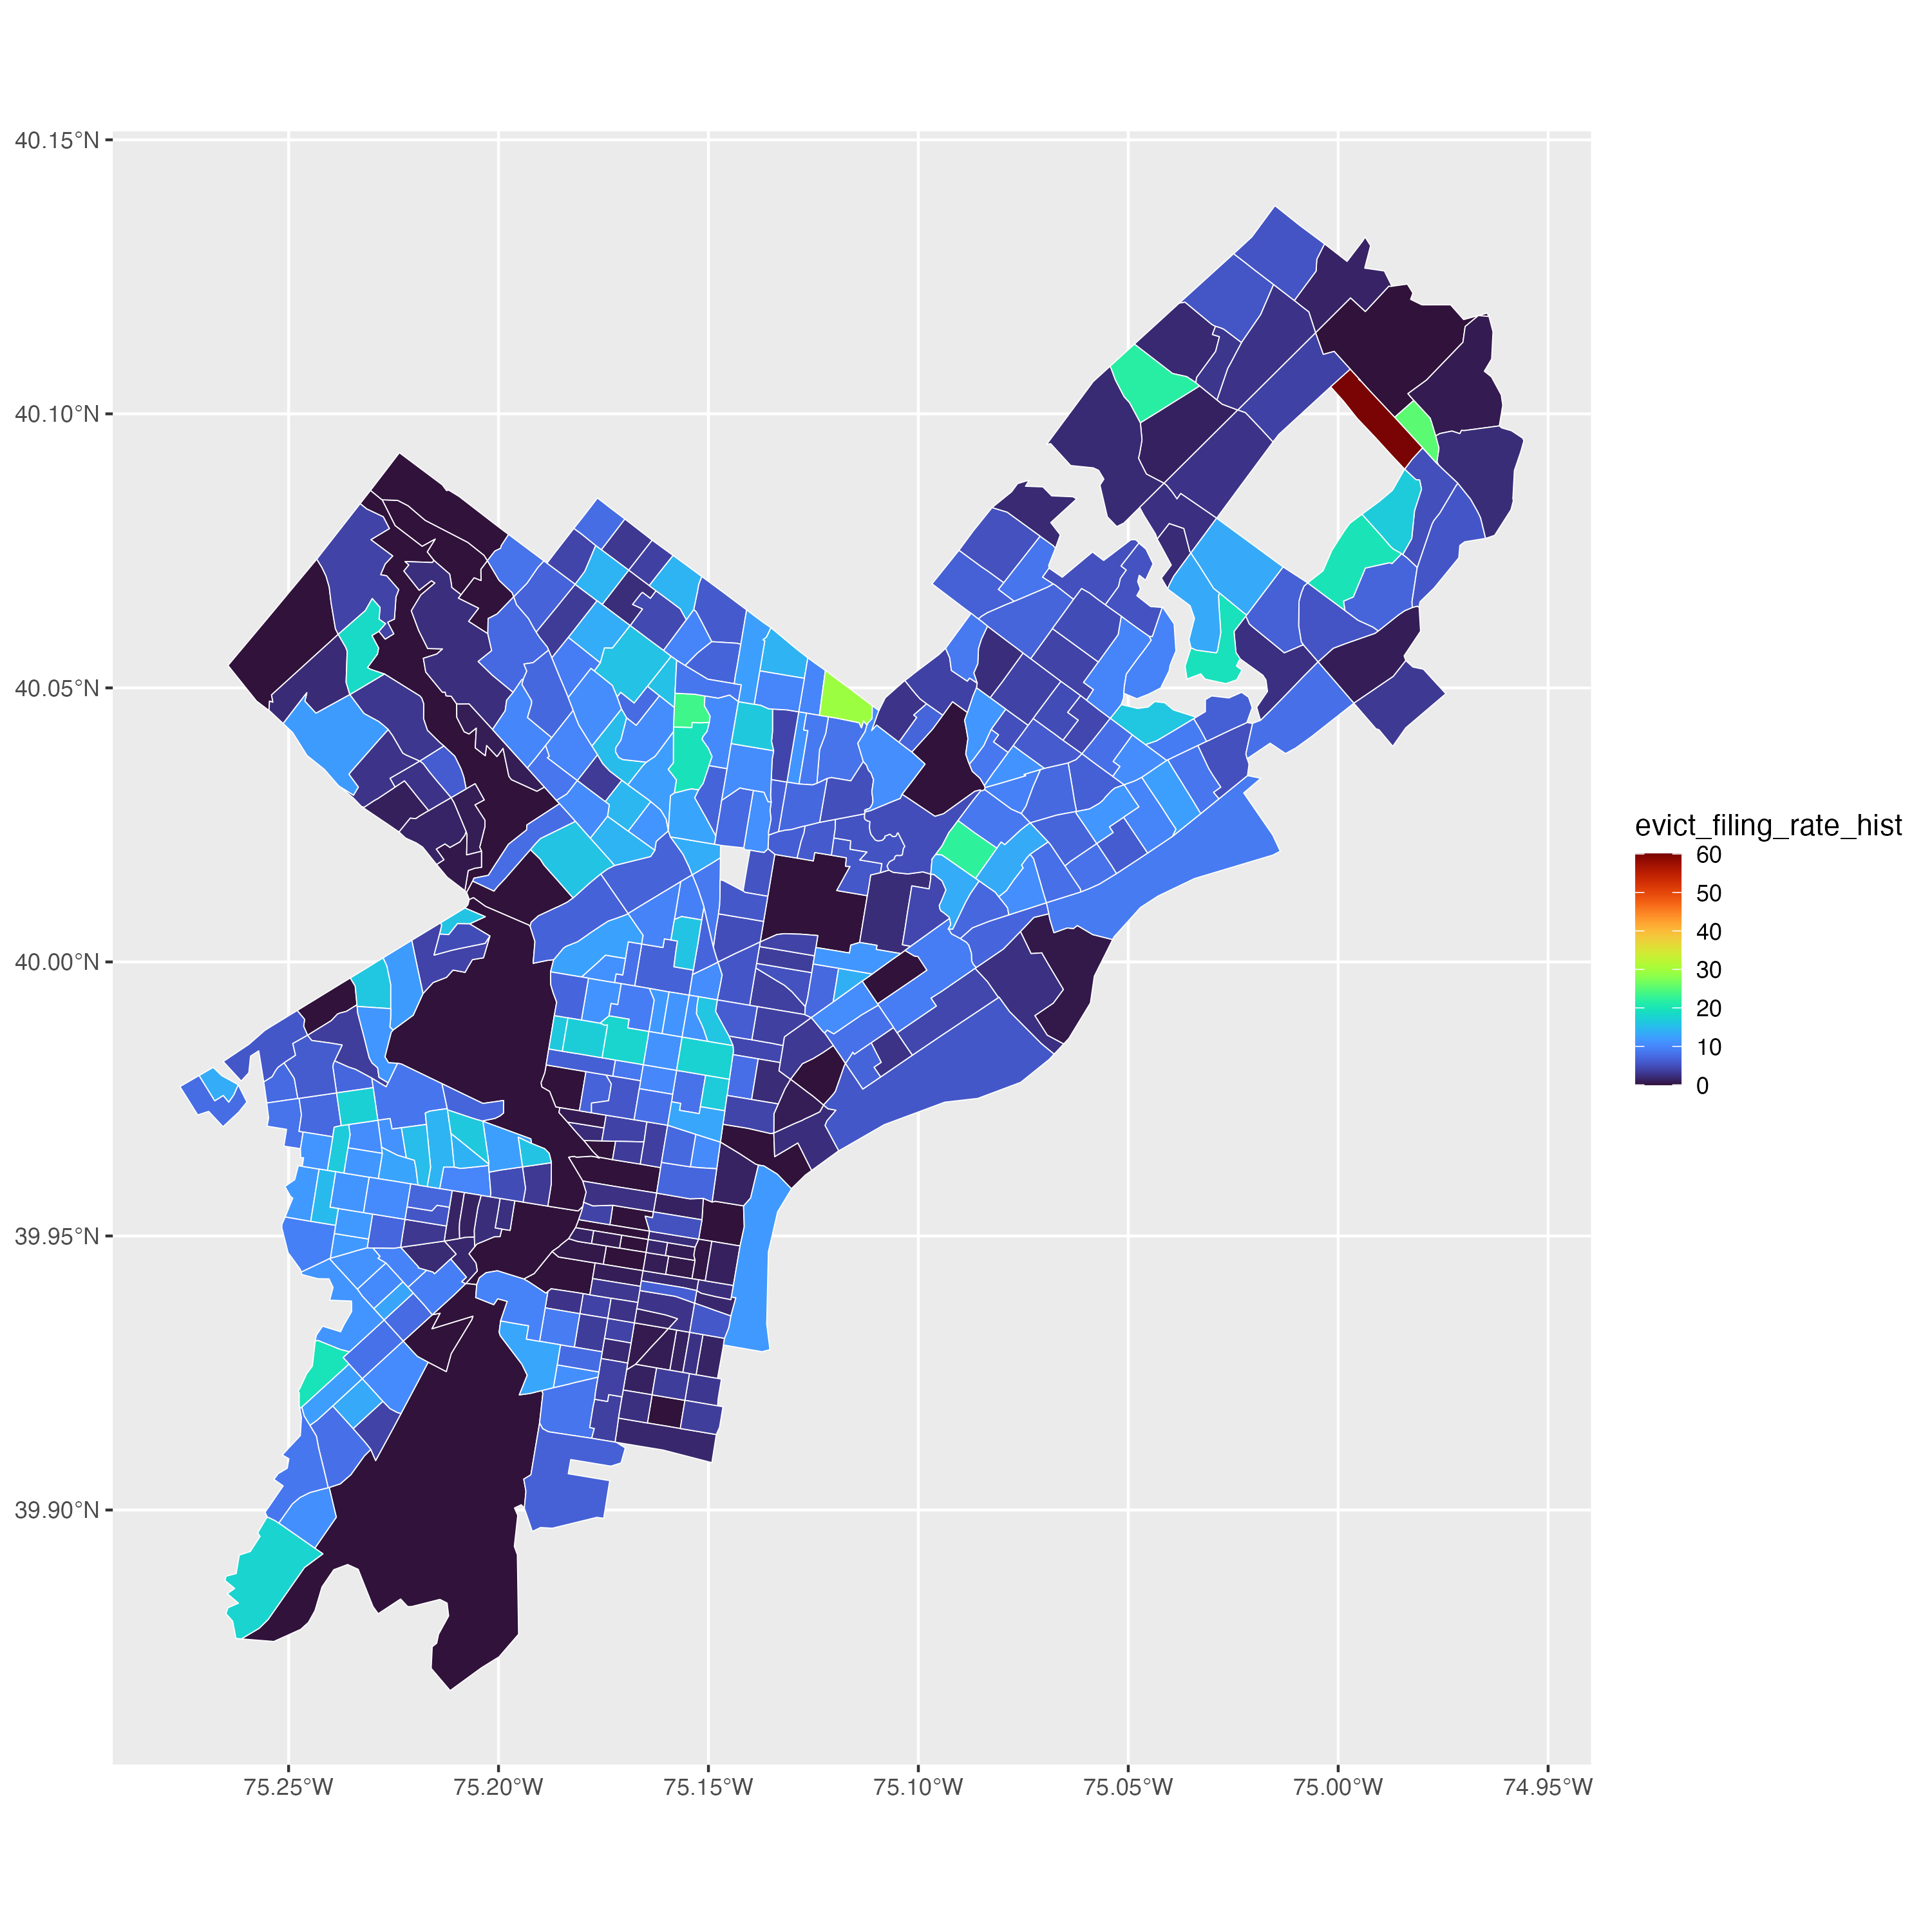
\includegraphics[width=0.6\linewidth]{figs/evict_filing_rate_hist.png}
    \caption{Evictions in Philadelphia}
    \label{fig:philly-map}
\end{figure}
    
\end{frame}

\begin{frame}{Evictions in Philadelphia: Tracts}
\begin{figure}
    \centering
    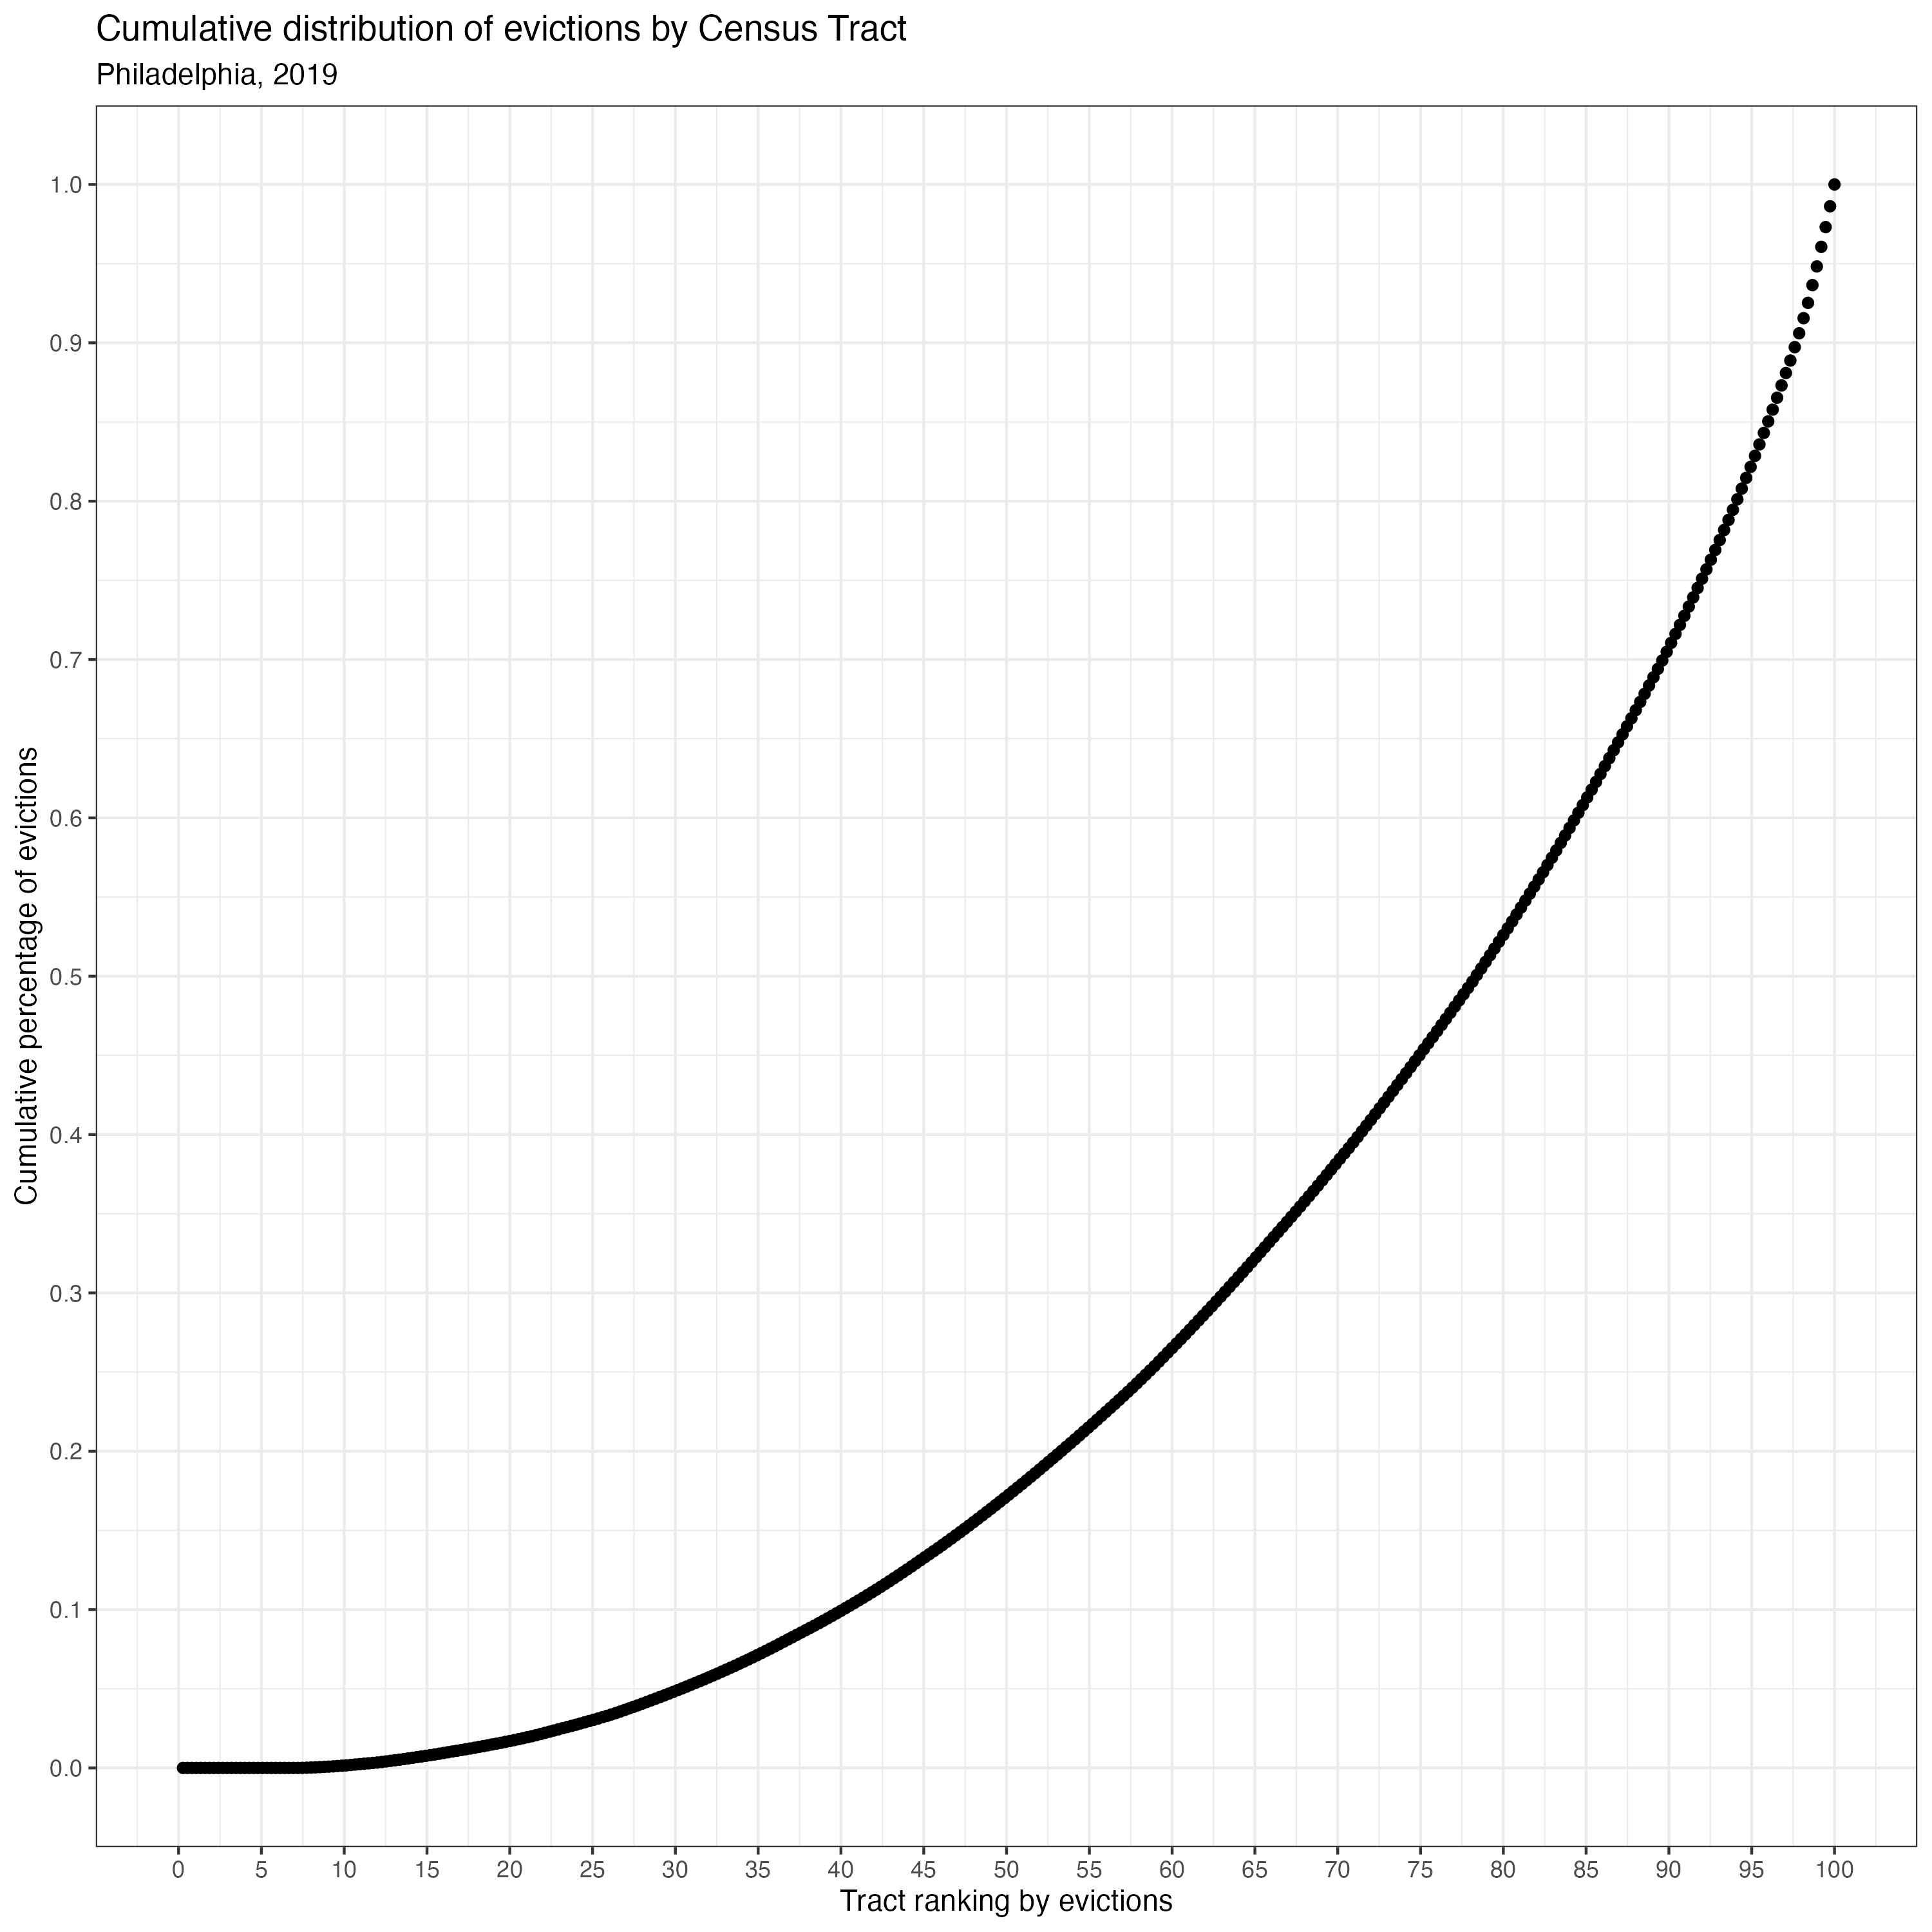
\includegraphics[width=0.6\linewidth]{figs/cumulative_evict_dist.png}
    \caption{CDF of Evictions by Census Tract}
    \label{fig:cum-tract}
\end{figure}
    
\end{frame}

\begin{frame}{Evictions in Philadelphia: Addresses}
\begin{figure}
    \centering
    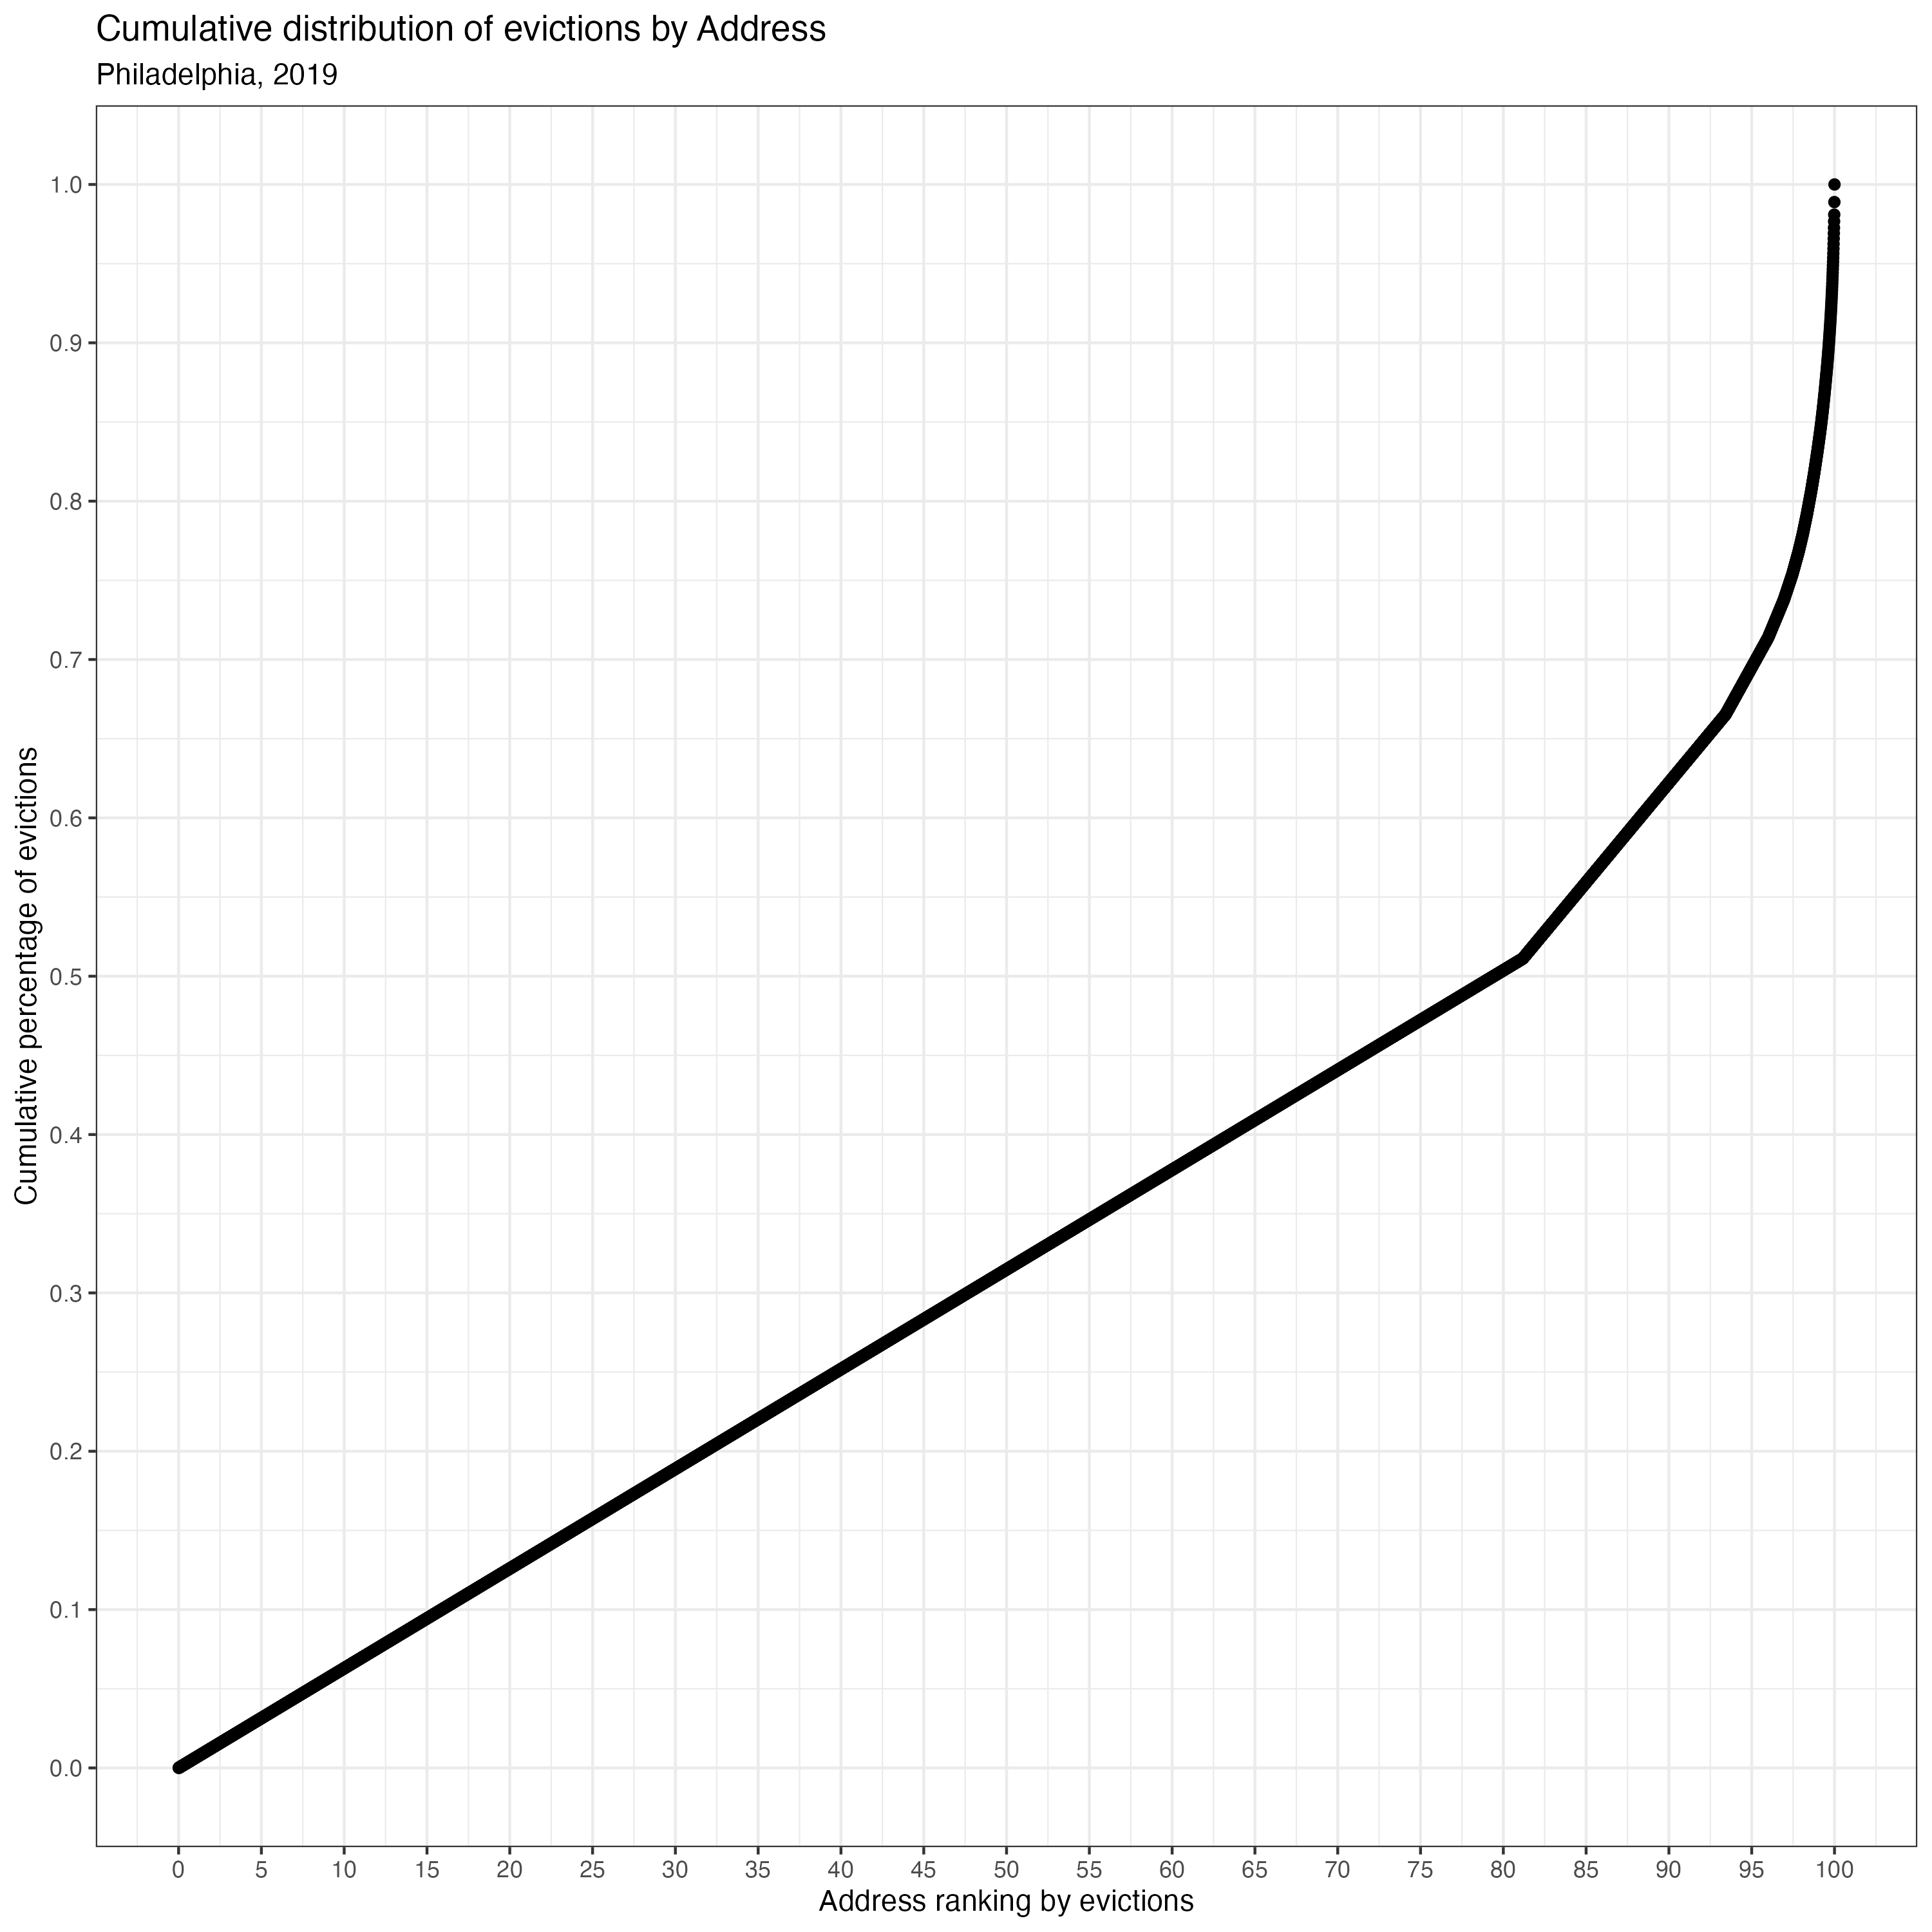
\includegraphics[width=0.6\linewidth]{figs/cumulative_evict_dist_address_hist.png}
    \caption{CDF of Evictions by Address}
    \label{fig:cum-address}
\end{figure}
    
\end{frame}

\begin{frame}{Evictions in Philadelphia: Plaintiffs}
\begin{figure}
    \centering
    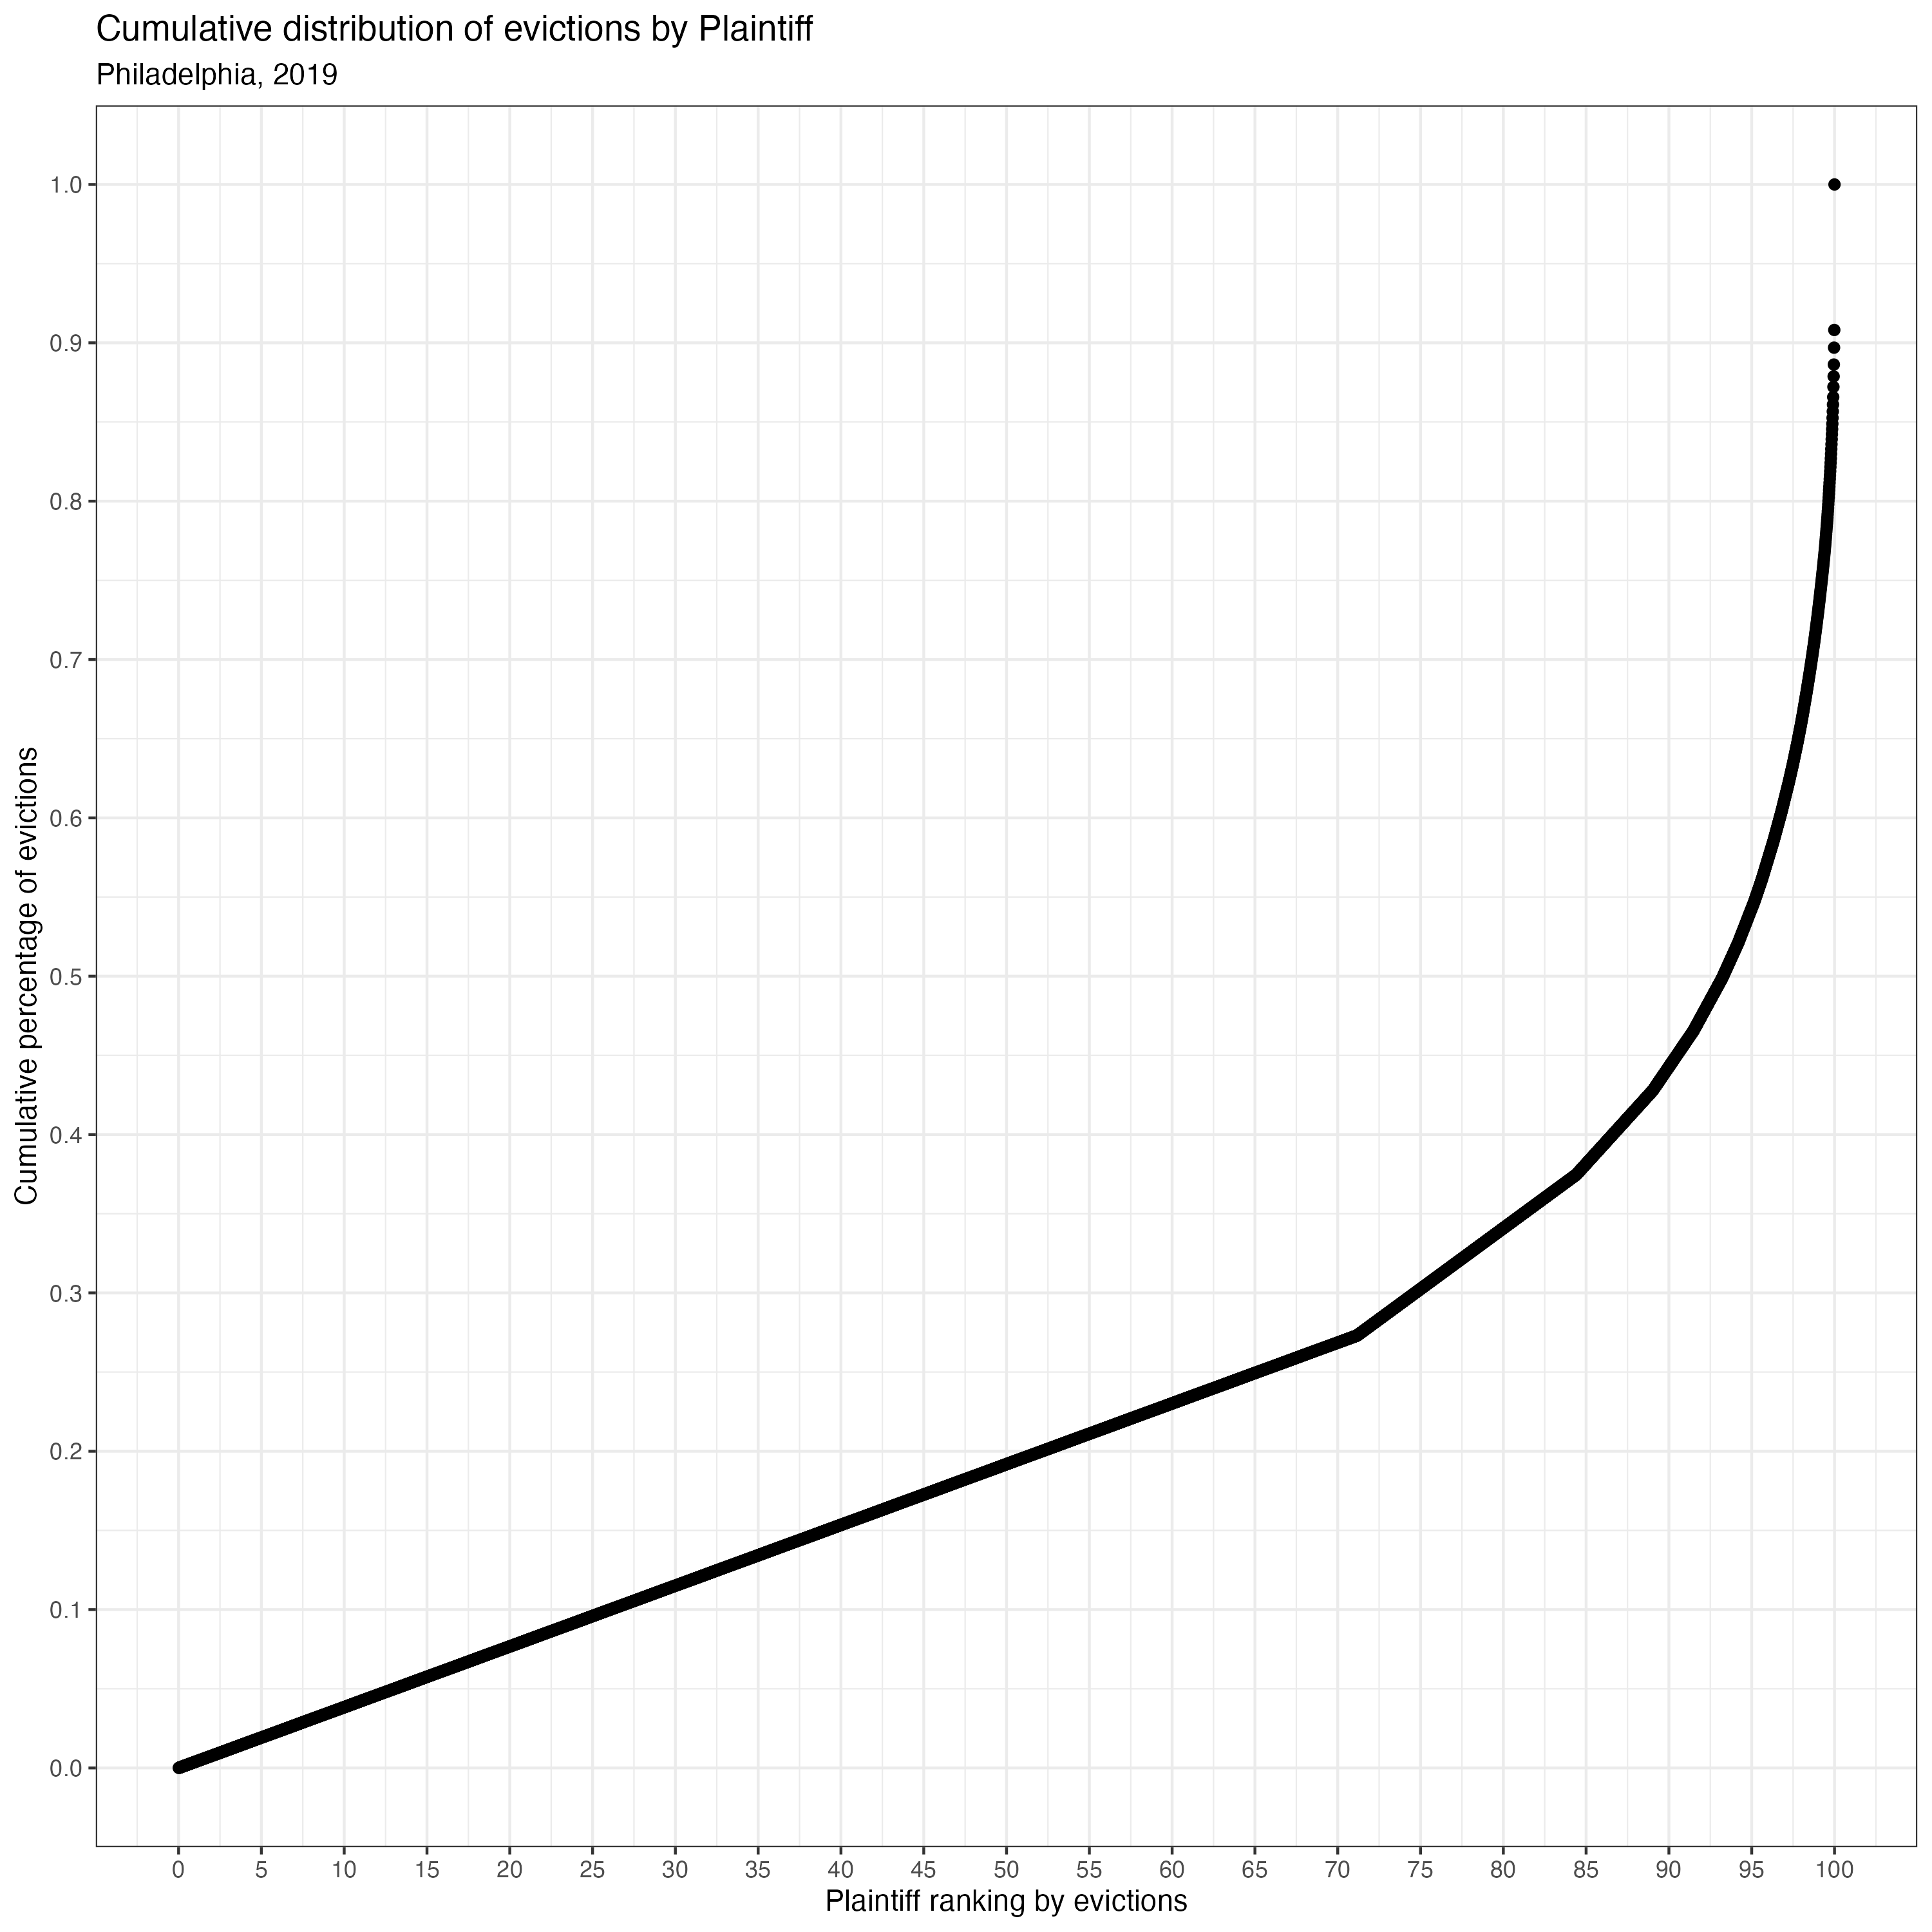
\includegraphics[width=0.6\linewidth]{figs/cumulative_evict_dist_plaintiff_hist.png}
    \caption{CDF of Evictions by Plaintiff Name}
    \label{fig:cdf-plaintiff}
\end{figure}
    
\end{frame}

\begin{frame}{Project to-dos}
\begin{itemize}
    \item Was the decline in evictions actually because of the program? (and did the program make removing tenants harder or did it just make removals not go through the court system)
    \item Assuming landlords can no longer evict with as much ease, how might they respond? Increase upfront discrimination? Renovate properties? Exit Market?
    \item Do effects seem large enough to justify a project?
\end{itemize}
    
\end{frame}

\end{document}
